\documentclass{bmstu}
\usepackage{pdfpages}
\usepackage{multirow}

% \usepackage{cmap} % Улучшенный поиск русских слов в полученном pdf-файле
\usepackage[T2A]{fontenc} % Поддержка русских букв
\usepackage[utf8]{inputenc} % Кодировка utf8
\usepackage[english,russian]{babel} % Языки: английский, русский
\usepackage{enumitem}
\usepackage{svg}

\usepackage{multirow}
\usepackage{threeparttable}

\usepackage[14pt]{extsizes}

\usepackage{caption}
\captionsetup[table]{justification=raggedright,singlelinecheck=off}
\captionsetup[lstlisting]{justification=raggedright,singlelinecheck=off}
\captionsetup{labelsep=endash}
\captionsetup[figure]{name={Рисунок}}

\usepackage{amsmath}
\usepackage{csvsimple}
\usepackage{enumitem} 
\setenumerate[0]{label=\arabic*)} % Изменение вида нумерации списков
\renewcommand{\labelitemi}{---}

\usepackage{geometry}
\geometry{left=30mm}
\geometry{right=15mm}
\geometry{top=20mm}
\geometry{bottom=20mm}

\usepackage{titlesec}
\titleformat{\section}{\normalsize\bfseries}{\thesection}{1em}{}
\titlespacing*{\chapter}{0pt}{-30pt}{8pt}
\titlespacing*{\section}{\parindent}{*4}{*4}
\titlespacing*{\subsection}{\parindent}{*4}{*4}

\usepackage{titlesec}
\titleformat{\chapter}{\LARGE\bfseries}{\thechapter}{16pt}{\LARGE\bfseries}
\titleformat{\section}{\Large\bfseries}{\thesection}{16pt}{\Large\bfseries}

\usepackage{setspace}
\onehalfspacing % Полуторный интервал

% Список литературы
\makeatletter 
\def\@biblabel#1{#1. } % Изменение нумерации списка использованных источников
\makeatother

\frenchspacing
\usepackage{indentfirst} % Красная строка после заголовка
\setlength\parindent{1.25cm}

\usepackage{ulem} % Нормальное нижнее подчеркивание
\usepackage{hhline} % Двойная горизонтальная линия в таблицах
\usepackage[figure,table]{totalcount} % Подсчет изображений, таблиц
\usepackage{rotating} % Поворот изображения вместе с названием
\usepackage{lastpage} % Для подсчета числа страниц

% Дополнительное окружения для подписей
\usepackage{array}
\newenvironment{signstabular}[1][1]{
	\renewcommand*{\arraystretch}{#1}
	\tabular
}{
	\endtabular
}

\usepackage{listings}
\usepackage{xcolor}

% Для листинга кода:
\lstset{%
	language=c++,   					% выбор языка для подсветки	
	basicstyle=\small\sffamily,			% размер и начертание шрифта для подсветки кода
	numbersep=5pt,
	numbers=left,						% где поставить нумерацию строк (слева\справа)
	%numberstyle=,					    % размер шрифта для номеров строк
	stepnumber=1,						% размер шага между двумя номерами строк
	xleftmargin=17pt,
	showstringspaces=false,
	numbersep=5pt,						% как далеко отстоят номера строк от подсвечиваемого кода
	frame=single,						% рисовать рамку вокруг кода
	tabsize=4,							% размер табуляции по умолчанию равен 4 пробелам
	captionpos=t,						% позиция заголовка вверху [t] или внизу [b]
	breaklines=true,					
	breakatwhitespace=true,				% переносить строки только если есть пробел
	escapeinside={\#*}{*)},				% если нужно добавить комментарии в коде
	backgroundcolor=\color{white}
}

\lstset{
	literate=
	{а}{{\selectfont\char224}}1
	{б}{{\selectfont\char225}}1
	{в}{{\selectfont\char226}}1
	{г}{{\selectfont\char227}}1
	{д}{{\selectfont\char228}}1
	{е}{{\selectfont\char229}}1
	{ё}{{\"e}}1
	{ж}{{\selectfont\char230}}1
	{з}{{\selectfont\char231}}1
	{и}{{\selectfont\char232}}1
	{й}{{\selectfont\char233}}1
	{к}{{\selectfont\char234}}1
	{л}{{\selectfont\char235}}1
	{м}{{\selectfont\char236}}1
	{н}{{\selectfont\char237}}1
	{о}{{\selectfont\char238}}1
	{п}{{\selectfont\char239}}1
	{р}{{\selectfont\char240}}1
	{с}{{\selectfont\char241}}1
	{т}{{\selectfont\char242}}1
	{у}{{\selectfont\char243}}1
	{ф}{{\selectfont\char244}}1
	{х}{{\selectfont\char245}}1
	{ц}{{\selectfont\char246}}1
	{ч}{{\selectfont\char247}}1
	{ш}{{\selectfont\char248}}1
	{щ}{{\selectfont\char249}}1
	{ъ}{{\selectfont\char250}}1
	{ы}{{\selectfont\char251}}1
	{ь}{{\selectfont\char252}}1
	{э}{{\selectfont\char253}}1
	{ю}{{\selectfont\char254}}1
	{я}{{\selectfont\char255}}1
	{А}{{\selectfont\char192}}1
	{Б}{{\selectfont\char193}}1
	{В}{{\selectfont\char194}}1
	{Г}{{\selectfont\char195}}1
	{Д}{{\selectfont\char196}}1
	{Е}{{\selectfont\char197}}1
	{Ё}{{\"E}}1
	{Ж}{{\selectfont\char198}}1
	{З}{{\selectfont\char199}}1
	{И}{{\selectfont\char200}}1
	{Й}{{\selectfont\char201}}1
	{К}{{\selectfont\char202}}1
	{Л}{{\selectfont\char203}}1
	{М}{{\selectfont\char204}}1
	{Н}{{\selectfont\char205}}1
	{О}{{\selectfont\char206}}1
	{П}{{\selectfont\char207}}1
	{Р}{{\selectfont\char208}}1
	{С}{{\selectfont\char209}}1
	{Т}{{\selectfont\char210}}1
	{У}{{\selectfont\char211}}1
	{Ф}{{\selectfont\char212}}1
	{Х}{{\selectfont\char213}}1
	{Ц}{{\selectfont\char214}}1
	{Ч}{{\selectfont\char215}}1
	{Ш}{{\selectfont\char216}}1
	{Щ}{{\selectfont\char217}}1
	{Ъ}{{\selectfont\char218}}1
	{Ы}{{\selectfont\char219}}1
	{Ь}{{\selectfont\char220}}1
	{Э}{{\selectfont\char221}}1
	{Ю}{{\selectfont\char222}}1
	{Я}{{\selectfont\char223}}1
}

\usepackage{pgfplots}
\usetikzlibrary{datavisualization}
\usetikzlibrary{datavisualization.formats.functions}

\usepackage{graphicx}
\newcommand{\imgScale}[3] {
	\begin{figure}[h!]
		\center{\includegraphics[scale=#1]{img/#2}} % height
		\caption{#3}
		\label{img:#2}
	\end{figure}
}

\newcommand{\imgHeight}[3] {
	\begin{figure}[h!]
		\center{\includegraphics[height=#1]{img/#2}} % height
		\caption{#3}
		\label{img:#2}
	\end{figure}
}

\usepackage[justification=centering]{caption} % Настройка подписей float объектов

\usepackage[unicode,pdftex]{hyperref} % Ссылки в pdf
\hypersetup{hidelinks}

\newcommand{\code}[1]{\texttt{#1}}

\bibliography{biblio}
\def\labelitemi{---}

\begin{document}
	
	\makeresearchtitle
    {Информатика и системы управления} % Название факультета
    {Программное обеспечение ЭВМ и информационные технологии} % Название кафедры
    {Методы распознавания лиц в видеопотоке} % Тема работы
    {Мамврийский~И.~С./ИУ7-56Б,Барсков~А.~Д./ИУ7-56Б, Салаев~Ю.~Д./ИУ7-56Б,Зайцев~К.~А./ИУ7-56Б} % Номер группы/ФИО студента (если авторов несколько, их необходимо разделить запятой)
    {Кострицкий~А.~С.} % ФИО научного руководителя
    {} % ФИО консультанта (необязательный аргумент; если консультантов несколько, их необходимо разделить запятой)
	
	\setcounter{page}{3}
    \maketableofcontents
	\chapter*{ВВЕДЕНИЕ}
\addcontentsline{toc}{chapter}{ВВЕДЕНИЕ}

В настоящее время, с ростом интереса к развитию технологий идентификации 
личности, особенно на основе изображений лиц, алгоритмы распознавания лиц 
приобретают все большее значение. Одним из ключевых направлений в области 
биометрических методов стало автоматическое обнаружение и идентификация 
лиц на изображениях, обеспечивая эффективные решения для таких 
разнообразных областей, как охранные системы, криминалистическая 
экспертиза, верификация, телеконференции, а также в сфере фотографии для 
автоматической фокусировки на лице человека.

Технология распознавания лиц на изображениях предоставляет преимущество 
перед другими биометрическими методами, поскольку не требует физического 
контакта с устройством. С учетом стремительного развития цифровой техники, 
она является наиболее приемлемой для массового применения. Однако, 
несмотря на свою эффективность, алгоритмы распознавания лиц сталкиваются 
с вызовами, такими как зависимость качества результата от условий 
освещенности, ракурса и положения лица, что требует постоянного 
совершенствования и анализа современных методов в данной области.

Цель данной работы --- описание методов распознавания лиц в 
видеопотоке.

В рамках выполнения работы необходимо решить следующие задачи:

\begin{itemize}[label=---]
  \item провести анализ предметной области;
  \item провести классификацию подходов к решению;
  \item провести анализ методов.
\end{itemize}


	\chapter{Метод главных компонент}

\section*{Определения}

\textit{Собственный вектор матрицы} --- ненулевой вектор, умножение квадратной матрицы на который дает тот же вектор с числовым коэффициентом, называемым собственным значением~\cite{linal}.

\textit{Ковариационная матрица вектора} --- квадратная симметрическая матрица, элементами которой являются ковариации --- меры связанности всех возможных пар компонент вектора. Ковариация имеет отрицательное значение, если большие значения одной компоненты соответствуют меньшим значениям другой, и наоборот. Ковариация имеет положительное значение, если большие значения одной компоненты соответствуют большим значениям другой, и аналогично для меньших значений. Ковариация компоненты вектора самой с собой равна дисперсии \cite{teorver}. На \eqref{eq:covariance_matrix} представлен пример ковариационной матрицы для трех компонент, ковариация обозначена как Cov$(X_1, X_2)$, дисперсия обозначена как Var$(X_1, X_2)$.

\begin{equation}\label{eq:covariance_matrix}
	\Sigma = 
	\begin{bmatrix}
		\text{Var}(X_1) & \text{Cov}(X_1, X_2) & \text{Cov}(X_1, X_3) \\
		\text{Cov}(X_2, X_1) & \text{Var}(X_2) & \text{Cov}(X_2, X_3) \\
		\text{Cov}(X_3, X_1) & \text{Cov}(X_3, X_2) & \text{Var}(X_3) \\
	\end{bmatrix}
\end{equation}

\section*{Алгоритм метода главных компонент}

Метод главных компонент --- один из статистических методов уменьшения размерности данных, т.~е. числа параметров, которые заданы переменными и необходимы для описания объекта. Такие методы по возможности сохраняют наибольшее количество информации и общую структуру данных~\cite{orlov, polyak}. Далее будет изложен алгоритм уменьшения размерности из $n$ в $k$:

\begin{enumerate}[label=\arabic*.]
	\item Метод главных компонент очень чувствителен к статистическим выбросам и неточностям в данных, поэтому перед применением необходима стандартизация данных --- приведение данных к единому масштабу~\cite{polyak, zakaria}. Это можно сделать вычитанием среднего из каждой переменной и делением полученного на стандартное отклонение \cite{zakaria}:
	
	\begin{equation}\label{eq:normalization_Z1}
		Z_i = \frac{{X_i - \bar{X_i}}}{{\sigma_{X_i}}}.
	\end{equation}
	\item Для уменьшения размерности данных необходимо найти переменные, которые сильно зависимы от значений друг друга, т.~е. cкоррелированные переменные. Это важно, поскольку такие переменные могут содержать излишнюю информацию, от которой можно было бы избавиться с минимальными потерями полезной информации. Чтобы понять, какие переменные скоррелированы, необходимо найти ковариационную матрицу.
	\item Далее необходимо найти главные компоненты --- новые переменные, которые получаются после введения новой системы координат таким образом, что каждая следующая главная компонента максимизирует дисперсию данных относительно себя, но не коррелирует с предыдущими главными компонентами, т.~е. перпендикулярна им. Таким образом, из $n$ изначальных переменных получится $n$ главных компонент, однако последним главным компонентам будет соответствовать наименьшая дисперсия, т.~е. наименьшая изменчивость --- это означает, что эти главные компоненты содержат наименьшее количество информации и могут быть отброшены с минимальными потерями. Математически направления осей главных компонент --- это собственные векторы ковариационной матрицы, а собственные значения --- это коэффициенты, отражающие дисперсию, соответствующую этой главной компоненте. Таким образом, полученные собственные значения необходимо упорядочить по убыванию и выбрать $k$ первых собственных векторов, которые и будут новыми переменными для уменьшения размерности~\cite{orlov, polyak, zakaria}.
	
	\begin{minipage}{\linewidth}
		\centering
		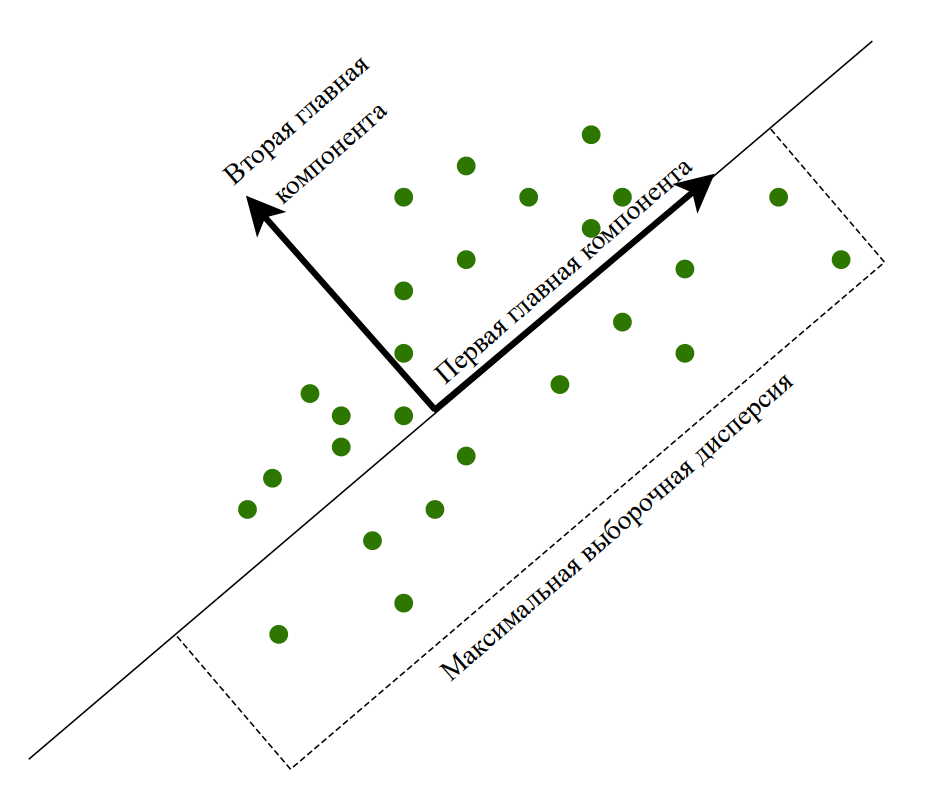
\includegraphics[width=0.9\textwidth]{img/pca1.png} 
		\captionof{figure}{Пример ввода первой и второй главных компонент}
		\label{fig:pca1}
	\end{minipage}

	
	\item На последнем шаге необходимо преобразовать данные, перейдя от исходных переменных к полученным $k$ главным компонентам. Для этого необходимо умножить транспонированную матрицу исходных данных $D$ на транспонированную матрицу главных компонент $PC$~\cite{zakaria}.
	
	\begin{equation}\label{eq:matrix_multiply}
		D^T \cdot PC^T
	\end{equation}
\end{enumerate}

\section*{Применение метода главных компонент для распознавания лиц}

Для задачи распознавания человека по изображению лица метод можно применить следующим образом: входные вектора представляют собой отцентрированные (лицо должно находиться в центре изображения и занимать большую его площадь) и приведённые к единому масштабу черно-белые изображения лица $m$ на $n$ пикселов. Собственные вектора, вычисленные для всего набора изображений лиц, называются собственными лицами ($eigenfaces$). Метод главных компонент в применении к изображениям лиц так же называют методом собственных лиц. Собственные лица имеют полезное свойство, заключающееся в том, что изображение, соответствующее каждому такому вектору имеет лицеподобную форму~\cite{brilyuk, parshin}.

\begin{figure}[h]
	\centering
	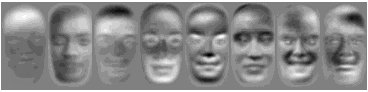
\includegraphics[width=0.85\textwidth]{img/pca2.png} 
	\caption{Пример собственных лиц~\cite{brilyuk}}
	\label{fig:pca2}
\end{figure}

Полученный один раз на обучающей выборке изображений лиц набор собственных векторов используется для кодирования всех остальных изображений лиц, которые представляются взвешенной комбинацией этих собственных векторов~\cite{parshin}. Процесс распознавания заключается в сравнении главных компонент неизвестного изображения с компонентами всех остальных изображений. Для этого обычно применяют какую-либо метрику (простейший случай --- Евклидово расстояние)~\cite{brilyuk}. 
	
	\chapter{Метод опорных векторов}
\section*{Введение}
В данном разделе рассмотрены основные понятия метода опорных векторов и алгоритм его работы. 
Определения терминов, используемых в данной работе.
\begin{enumerate}
	\item Гиперплоскость – это $(n-1)$-мерная подплоскость в $n$-мерном евклидовом пространстве, которая разделяет пространство на две отдельные части \cite{hyperploskostb}.
	\item Ядро – это функция, которая вычисляет точечное произведение двух векторов в высокоразмерном пространстве \cite{kernel}.
	\item Радиальные базисные функции – это класс функций, которые используются в нейронных сетях для аппроксимации и интерполяции данных \cite{rbf}.
\end{enumerate}

\section*{Основная часть}

Метод опорных векторов – линейный алгоритм, который используется в задачах классификации и регрессии. 
Суть алгоритма – найти линию или гиперплоскость, разделяющую данные на классы.

Изначально метод опорных векторов работает как линейный классификатор, способный решать только задачи, где классы данных можно разделить прямой линией. 
Однако при использовании нелинейных ядер, метод опорных векторов способен преобразовывать исходные данные в пространство более высокой размерности, где можно найти оптимальную разделяющую гиперплоскость \cite{all}. 
Некоторые из популярных ядер метода опорных векторов:
\begin{itemize}
	\item линейное ядро (преобразует данные в ту же размерность без изменений);
	\item полиномиальное ядро (преобразует данные в более высокую размерность с использованием полиномиальной функции);
	\item радиальное базисное функциональное ядро (преобразует данные в бесконечно высокую размерность с использованием радиальной базисной функции).
\end{itemize}

Пример. На рисунке \ref{pic_1} изображен набор данных, который необходимо классифицировать и отделить квадраты от треугольников. Существует бесконечное количество линий, способных разделить эти два класса. Основная цель в поставленной задаче – найти оптимальную из них.

\begin{figure} [H]
	\centering{
		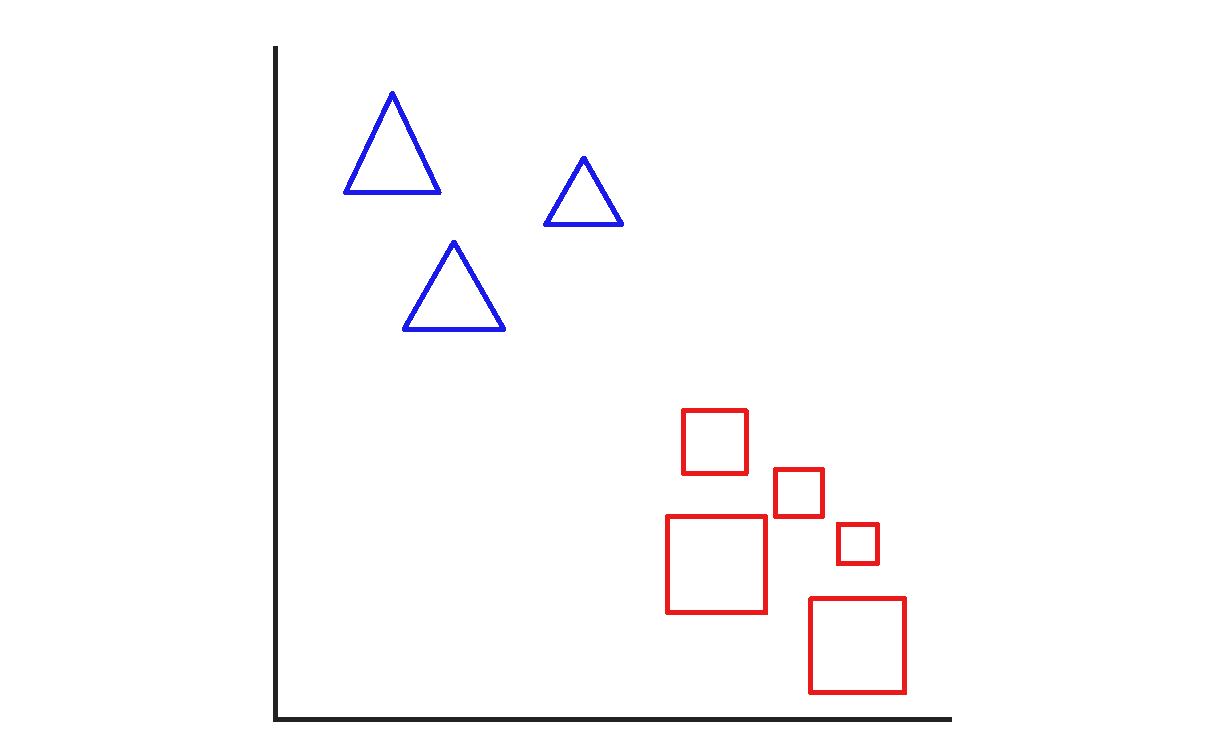
\includegraphics[scale=0.7]{img/circles.pdf}
		\caption{Исходные данные}
		\label{pic_1}
	}
\end{figure}

На рисунке \ref{pic_2} изображены два варианта разделения на классы.

\begin{figure} [H]
	\centering{
		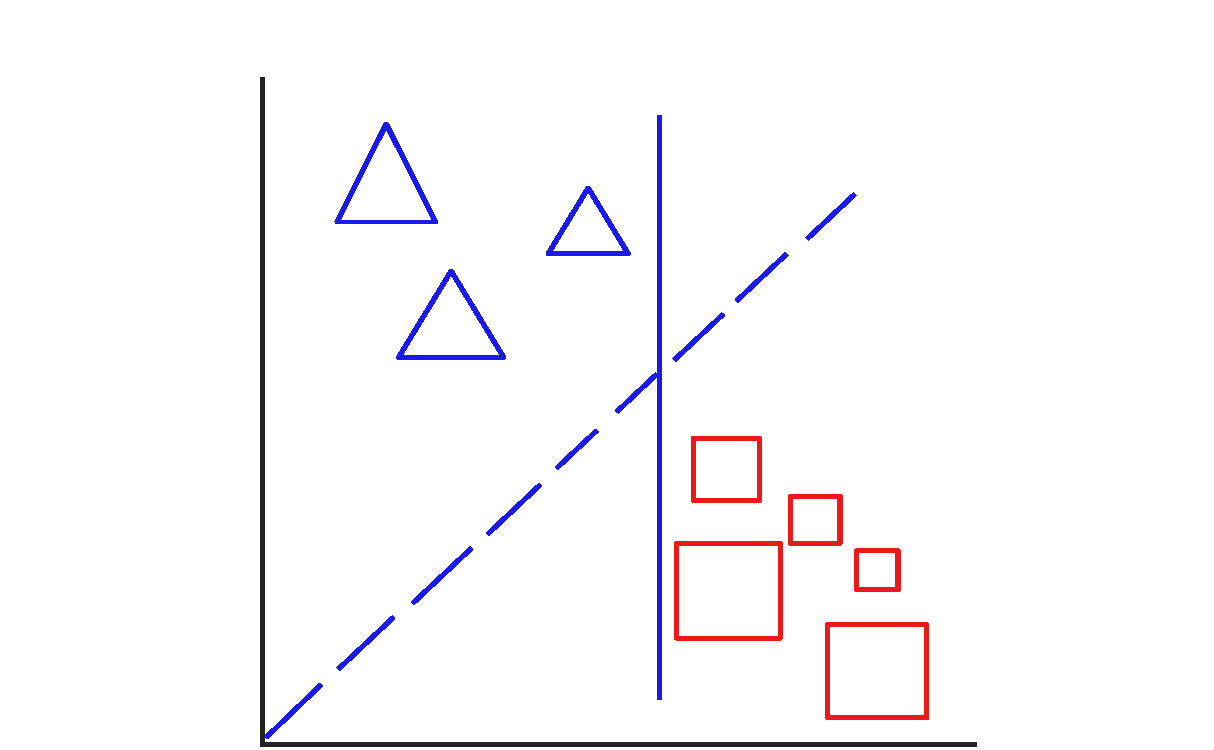
\includegraphics[scale=0.7]{img/circles2.pdf}
		\caption{Варианты разделяющих линий}
		\label{pic_2}
	}
\end{figure}

Сплошная линия проходит слишком близко к классам треугольников и квадратов. Несмотря на то, что она верно классифицировала все объекты текущего набора данных, она не будет генерализованной, не будет так же хорошо разграничивать незнакомый набор данных. Поэтому в данном случае оптимальные выбор -- прерывистая линия \cite{all}.

Основные этапы метода опорных векторов.
\begin{enumerate}[label=\arabic*.]
	\item Подготовка обучающего набора данных, состоящего из пар (вектор признаков, метка класса).
	\item Выбор ядра и настройка параметров модели.
	\item Минимизация функции потерь с использованием оптимизационных методов для нахождения гиперплоскости, максимально разделяющей классы.
	\item Нахождение опорных векторов (опорные векторы -- точки данных, лежащие на границах зазора между классами).
	\item Определение гиперплоскости: гиперплоскость строится для максимизации зазора между классами с учетом опорных векторов и параметров ядра.
	\item Оценка обобщающей способности модели на тестовой выборке для проверки ее работоспособности на новых данных.
\end{enumerate}

	\chapter{Метод Виолы-Джонса}

Метод Виолы--Джонса --- алгоритм, позволяющий обнаруживать и распознавать лица на изображениях и видеопоследовательностях в режиме реального времени ~\cite{viola}. Данный метод основан на использовании следующих принципов:
\begin{enumerate}[label=\arabic*.]
    \item Интегральное представление изображения

    Представим исходное изображение в виде матрицы, каждый элемент которой содержит значение интенсивности пикселя. Интегральное представление изображения формируется путем создания новой матрицы, размерность которой совпадает с матрицей исходного изображения. В каждом элементе данной матрицы хранится сумма интенсивностей всех пикселей исходного изображения, находящихся левее и выше текущего пикселя в исходной матрице ~\cite{tomsk}, т. е. элементы новой матрицы рассчитываются по следующей формуле:
    
    \begin{equation}
        L(x,y) = \sum_{i=0, j=0}^{i<=x, j<=y} I(i,j),
    \end{equation}

    где $I(i, j)$ --- значение элемента матрицы исходного изображения, $L(x,y)$ --- значение элемента матрицы интегрального изображения.

    Особенностью интегрального представления является возможность вычисления суммы интенсивностей пикселей внутри произвольных прямоугольных областей ~\cite{tomsk}. Рассмотрим следующий пример, где искомой областью является прямоугольник $ABCD$:

    \begin{figure}[h]
	\centering
	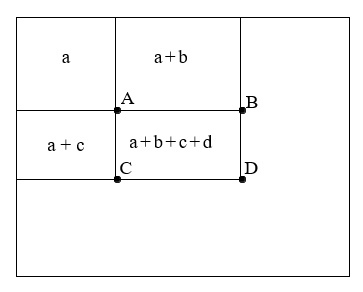
\includegraphics[height=0.25\textheight]{img/integral.jpg}
	\caption{Расчет суммы интенсивностей пикселей в прямоугольнике $ABCD$}
    \label{img:integral}
    \end{figure}

    Сумма интенсивностей пикселей, лежащих внутри области $ABCD$, будет вычисляться по следующей формуле:

    \begin{equation}
        F(ABCD) = F(A) + F(D) - F(B) - F(C),
    \end{equation}

    где $F(X)$ --- суммы интенсивностей пикселей внутри прямоугольной области X.

    Таким образом, для вычисления суммы интенсивностей пикселей внутри произвольных прямоугольных областей требуется четыре обращения к матрице интегрального представления изображения.
    
    \item Признаки Хаара

    Для выделения областей изображения, которые наиболее вероятно содержат нужные объекты, используются признаки Хаара. Признак Хаара --- результат сравнения смежных прямоугольных областей изображения путем вычисления разности сумм интенсивностей пикселей соответствующих прямоугольников ~\cite{novosibirsk}. 
    В методе Виолы~---~Джонса используются три вида данных признаков: <<два прямоугольника>>, <<три прямоугольника>>, <<четыре прямоугольника>> ~\cite{viola} (рис.~\ref{img:haar} ~\cite{astrahan}).

    \begin{figure}[h]
	\centering
	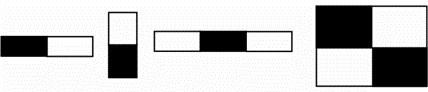
\includegraphics[height=0.1\textheight]{img/haar.jpg}
	\caption{Признаки Хаара}
    \label{img:haar}
    \end{figure}

    Значение каждого признака вычисляется по следующей формуле:

    \begin{equation}
        F = X - Y,
    \end{equation}

    где X - сумма интенсивностей пикселей, находящихся в светлой области признака, Y - сумма интенсивностей пикселей, находящихся в темной области признака.

    Для вычисления данных сумм интенсивностей пикселей за константное время используется интегральное представление изображения.
    
    \item Алгоритм AdaBoost

    Для прогнозирования категории, к которой относится входной объект, в машинном обучении используется модель, называемая классификатором ~\cite{classifier}. Слабый (или простой) классификатор —-- это классификатор, который решающий задачу классификации чуть лучше, чем случайное угадывание ~\cite{weak}, т. е. вероятность ошибки меньше 50\%. 

    Для повышения точности аналитических моделей используется бустинг (англ. boosting) --- последовательная композиция алгоритмов машинного обучения, в которой каждый следующий алгоритм стремится компенсировать недостатки композиции всех предыдущих алгоритмов ~\cite{tomsk}. 
    В методе Виолы~---~Джонса в качестве бустинга выбран алгоритм AdaBoost, в ходе выполнения которого формируется сложный классификатор, состоящий из набора простых и имеющий меньшую вероятность ошибки, чем у каждого слабого классификатора по отдельности:

    \begin{equation}
        a_s(x) = \sum_{i=1}^{n}b_i * a_i(x),
    \end{equation}

    где x --- изображение, $a_s(x)$ --- сложный классификатор, $a_i(x)$ --- слабый классификатор, $b_i$ --- весовой коэффициент соответствующего слабого классификатора.

    Основные этапы работы алгоритма AdaBoost ~\cite{viola}:

    \begin{itemize}
        \item Инициализация весов объектов обучающего набора одинаковым значением;
        \item Для каждой итерации алгоритма на основе сравнения ошибок классификации выбирается слабый классификатор, который наилучшим образом разделяет обучающий набор с учетом текущих весов объектов;
        \item Для каждого выбранного классификатора вычисляется его ошибка и вес, отражающий точность разделения объектов;
        \item Обновление весов объектов таким образом, чтобы неправильно классифицированые объекты получили больший вес на следующей итерации;
        \item Формирование сложного классификатора на основе слабых классификаторов и их весов.
    \end{itemize}
    
    Таким образом, в ходе выполнения данного алгоритма путем исключения большинства имеющихся признаков выбираются наиболее подходящие для конкретного объекта, в результате чего формируется классификатор с критическими признаками.

    В качестве классификаторов в методе Виолы~---~Джонса используются вышеописанные признаки Хаара. Для каждого признака выбирается соответствующий порог для бинарной классификации объектов, т. е. для определения того, какие значения признака считаются положительными, а какие --- отрицательными. Выбор оптимального порога осуществляется таким образом, чтобы минимизировать ошибку классификации, учитывая веса объектов в процессе обучения алгоритма.
    
    \item Каскадная структура классификаторов - последовательное объединение усложняющихся классификаторов в каскадную структуру (рис.~\ref{img:cascade} ~\cite{astrahan}) ~\cite{viola}. Данная структура повышает скорость обнаружения объектов, фокусируя свою работу на наиболее информативных областях изображения ~\cite{tomsk}. Это достигается тем, что каскад пытается отсеять как можно больше отрицательных экземпляров на самом раннем этапе: количество вычисленных признаков для анализа отрицательных областей должно быть значительно меньше, чем количество признаков, вычисленных для положительных областей. Следовательно, более сложные классификаторы применяются только к тем областям, которые уже прошли отсев более простыми классификаторами, что экономит ресурсы и улучшает производительность системы.

    \begin{figure}[h]
	\centering
	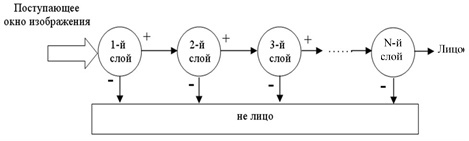
\includegraphics[width=120mm,height=0.17\textheight]{img/cascade.jpg}
	\caption{Каскадная структура классификаторов}
    \label{img:cascade}
    \end{figure}

    \item Сканирующее окно

    Для выделения областей, в которых могут находиться нужные объекты, используется сканирующее окно —-- перемещаемая прямоугольная активная область, в которой осуществляется поиск объектов ~\cite{tula}. Данный подход включает в себя пошаговый анализ различных прямоугольных подокон изображения, взятых с различными смещениями и масштабами. Впоследствии для каждой такой области применяются вышеописанные каскады классификаторов, которые оценивают, соответствует ли содержимое подокна определенным критериям.

\end{enumerate}

Алгоритм распознавания лиц:

\begin{enumerate}[label*=\arabic*.]
    \item Определить признаки Хаара.
    \item Сформировать обучающий набор и инициализировать веса объектов данного набора.
    \item Пока не достигнута заданная точность обучения:
    \begin{enumerate}
        \item Выбрать признак Хаара и порог, минимизирующие ошибку классификации при текущих весах.
        \item Вычислить вес полученного классификатора на основе ошибки классификации.
        \item Обновить веса объектов с учетом веса классификатора.
    \end{enumerate}
    \item Сформировать каскадную структуру из полученных классификаторов.
    \item Создать матрицу интегрального представления.
    \item Инициализировать сканирующее окно.
    \item Применить каскад классификаторов к текущему окну.
    \begin{enumerate}
        \item Если лицо обнаружено, то выделить эту область изображения, иначе продолжить проверку.
        \item Если не все окна проверены, то изменить параметры окна, иначе вернуть результаты обнаружения лиц.
    \end{enumerate}
\end{enumerate}
	\chapter{Метод гибкого сравнения на графах}

Метод гибкого сравнения на графах -- метод обработки изображений и распознавания образов, который 
используется для нахождения соответствия между двумя изображениями, учитывая возможные искажения, изменение масштаба и повороты~\cite{distances}.

Данный метод является одним из способов распознования лиц.
Лица представлены в виде графов со взвешенными
вершинами и ребрами\cite{wen}. 
Во время распознавания один из графов –- константный(эталонный), 
в то время как другой изменяется(деформируется) с 
целью наилучшей подгонки к первому. 

В данном методе графы могут представлять собой как 
прямоугольную решетку (рис. \ref{img:ant}.a), так и структуру, образованную антропометрическими
точками лица(рис. \ref{img:ant}.б).

\begin{figure}[h]
    \centering
    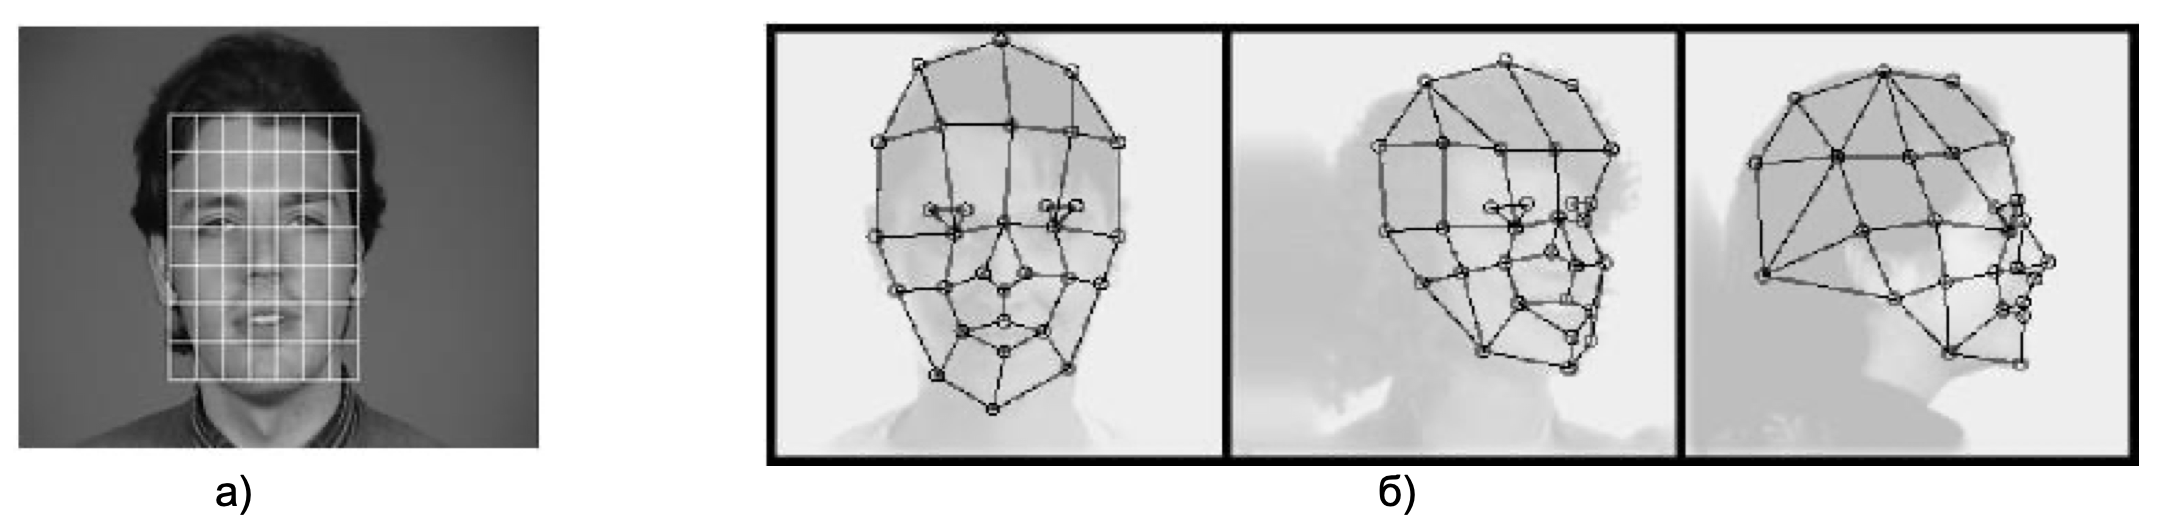
\includegraphics[height=0.15\textheight]{img/ex.jpg}
    \caption{Пример структуры графа для распознования лиц \\ 
    a)Регулярная решетка; \\ б)Граф на основе антропометрических точек лица.}
    \label{img:ant}
\end{figure}

Частотное содержимое изображения --- характеристика, показывающая насколько быстро 
меняется яркость или цвет в различных частях изображения~\cite{chst}.

Фильтр Габора --- фильтр, который анализирует, присутствует ли какое-либо конкретное частотное содержимое 
в изображении в различных направлениях в области вокруг точки или области анализа. Данный фильтр представляет собой 
синусоидальную плоскую волну(рис. \ref{img:sinuso}).\cite{gb}
\begin{figure}[h]
    \centering
    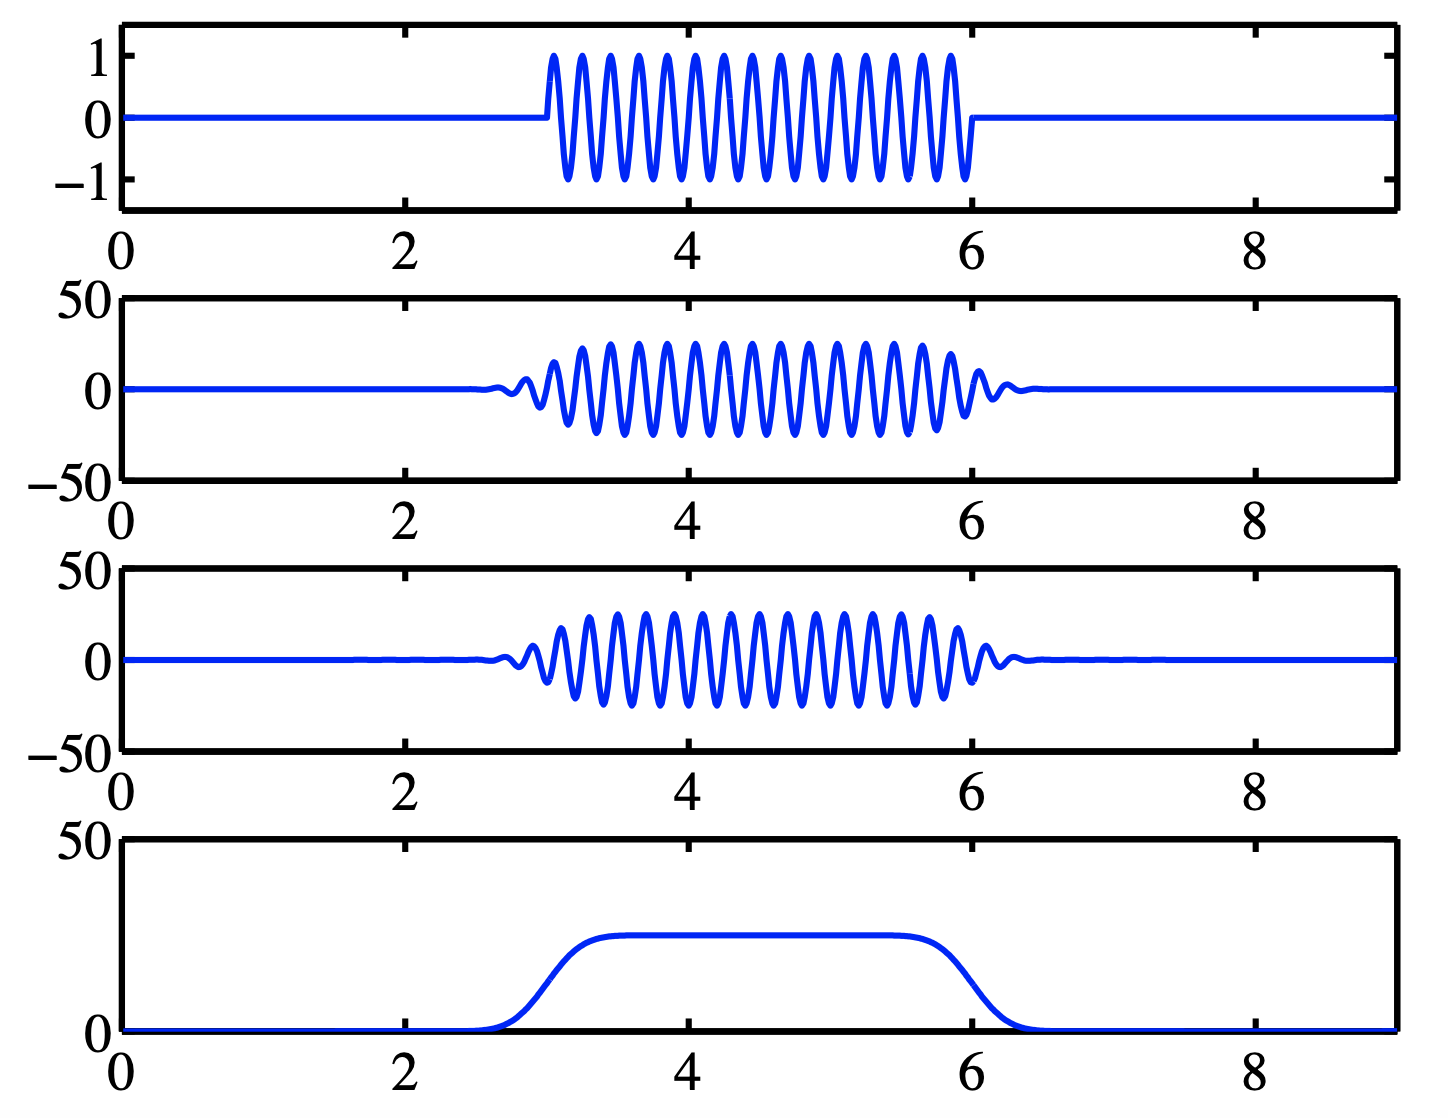
\includegraphics[width=0.35\textheight]{img/sin.png}
    \caption{Пример синусоидальной плоской волны.}
    \label{img:sinuso}
\end{figure}

\vspace{\baselineskip}
\vspace{\baselineskip}
\vspace{\baselineskip}
\vspace{\baselineskip}
\vspace{\baselineskip}
\vspace{\baselineskip}
\vspace{\baselineskip}

Свертка -- операция вычисления нового значения интенсивности, степени яркости
светлых пикселей по сравнению с более темными тонами,
заданного пикселя, при котором учитываются значения окружающих его соседних пикселей.

В некоторой локальной области вершины графа вычисляют значения
путем свертки значений яркости пикселей с набором(рис. \ref{img:gabnab}) фильтров Габора(рис. \ref{img:gab}).

\begin{figure}[h]
    \centering
    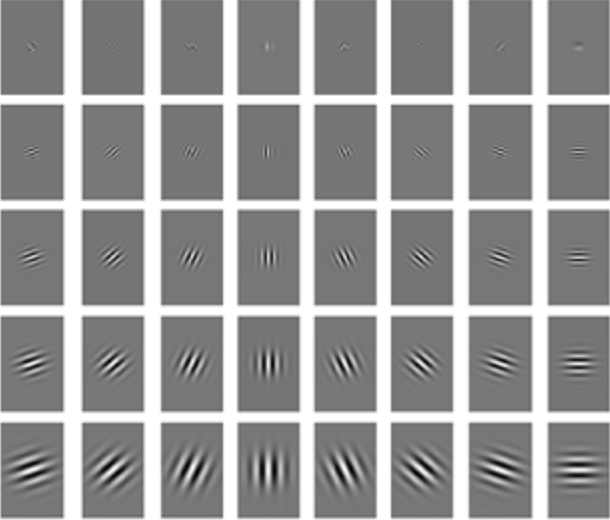
\includegraphics[height=0.35\textheight]{img/img_b.jpg}
    \caption{Набор фильтров Габора.}
    \label{img:gabnab}
\end{figure}
\vspace{\baselineskip}
\vspace{\baselineskip}
\vspace{\baselineskip}
\vspace{\baselineskip}
\vspace{\baselineskip}

\begin{figure}[h]
    \centering
    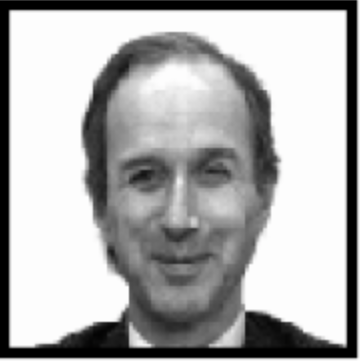
\includegraphics[height=0.15\textheight]{img/gbr1.png}
    
\includegraphics[height=0.15\textheight]{img/gbr2.png}
    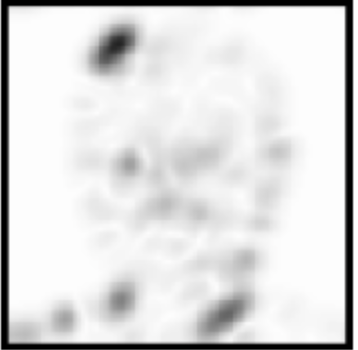
\includegraphics[height=0.15\textheight]{img/gbr3.png}
    \caption{Пример свертки изображения лица с фильтрами Габора.}
    \label{img:gab}
\end{figure}

\textbf{Алгоритм распознования лица:}
\begin{enumerate}
    \item Происходит деформация графа путем смещения каждой из его вершин на некоторое расстояние
    в различных направлениях относительно его исходного местоположения(рис. \ref{img:demonstration});
    \item Выбирается такая позиция, при которой разница между значениями в вершине деформируемого графа и 
    соответствующей ей вершине эталонного графа будет минимальной;
    \item Данная операция выполняется поочердено для всех вершин графа, пока не будет достигнуто наименьшее суммарное различие 
    между признаками этих графов;
    \item  Данная процедура деформации выполняется для всех эталонных лиц, заложенных в базу данных системы. 
    Результат распознавания -- эталон с наименьшим суммарным различием.
\end{enumerate}

\begin{figure}[h]
    \centering
    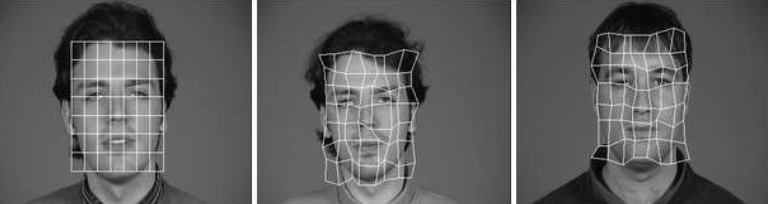
\includegraphics[height=0.15\textheight]{img/img_a.jpg}
    \caption{Пример деформации графа.}
    \label{img:demonstration}
\end{figure}
    

	\chapter{Классифкация методов распознования лиц в видеопотоке}

Методы распознавания лиц в видеопотоке можно классифицировать по различным критериям, например, по подходу к представлению данных, по типу обучения и по применению в задаче распознавания лиц. В таблице \ref{tab:table} представлена данная классификация.

\begin{table}[h]
    \centering
    \small
    \caption{\label{tab:table} Классификация методов распознования лиц в видеопотоке}
    \begin{tabular}{|p{2cm}|p{3cm}|p{5cm}|p{5cm}|}
        \hline
        \multicolumn{1}{|l|}{\textbf{Методы}} & \multicolumn{3}{c|}{\textbf{Классификация}} \\
        \cline{2-4}
        & \textbf{по типу обучения} & \textbf{по подходу к представлению данных} & \textbf{по применению в распознавании лиц} \\
        \hline
        Метод главных компонент & Без учителя (преобразование данных) & Использует проецирование изначальных данных на главные компоненты & Используется для снижения размерности признакового пространства при работе с изображениями лиц \\
        \hline
        Метод гибкого сравнения на графах & В зависимости от реализации, может быть как с учителем, так и без учителя & Использует графы для представления структурной информации о лицах & Используется при работе с изображениями, где важна структура и отношения между частями лица \\
        \hline
        Метод опорных векторов & С учителем (обучение с классифицированными примерами) & Использует векторы признаков для построения гиперплоскости, разделяющей классы & Используется в задачах классификации лиц, особенно в случаях, когда есть различные классы (например, различные люди) \\
        \hline
        Метод Виолы-Джонса & С учителем (обучение на положительных и отрицательных примерах) & Использует характеристики (признаки), основанные на интенсивности пикселей & Применяется для обнаружения лиц в реальном времени, основываясь на быстрых вычислениях признаков \\
        \hline
    \end{tabular}
\end{table}

	\chapter*{ЗАКЛЮЧЕНИЕ}
\addcontentsline{toc}{chapter}{ЗАКЛЮЧЕНИЕ}


Цель данной работы, которая заключалась в классификации методов распознавания лиц в 
видеопотоке, выполнена. 

В ходе выполнения данной работы были решены следующие задачи:
\begin{itemize}[label=---]
  \item проведен анализ предметной области распознавания лиц в видеопотоке;
  \item описаны методы распознавания лиц в видеопотоке;
  \item сформулированы критерии сравнения применяемых методов;
  \item выполнена классификация данных методов.
\end{itemize}



    \makebibliography

\end{document}
